\documentclass[10pt]{beamer}

\setbeamertemplate{footline}[page number]

\usepackage{tikz}

\newtheorem{conjecture}{Conjecture}

\DeclareFontFamily{U}{wncyr}{}
\DeclareFontShape{U}{wncyr}{m}{n}{<->wncyr10}{}
\DeclareSymbolFont{cyr}{U}{wncyr}{m}{n}
\DeclareMathSymbol{\Sha}{\mathord}{cyr}{"58}

\title{Hyperelliptic curves over function fields}
\subtitle{Study group on arithmetic of hyperelliptic curves}
\author{David Kurniadi Angdinata}
\institute{University College London}
\date{Friday, 28 November 2025}

\begin{document}

\frame{\titlepage}

\begin{frame}[t]{Global function fields}

A \emph{function field} $ F = k(C) $ is that of a \emph{nice} \footnote{smooth proper geometrically irreducible} curve $ C $ over a base field $ k $. When $ k = \mathbb{F}_q $ is a finite field of size $ q $, this is a \emph{global function field}.

\vspace{0.5cm} A \emph{ring of integers} $ \mathcal{O}_F $ of a global function field $ F $ is the ring of sections over an open affine $ U \subseteq C $, in which case $ C \setminus U $ are its \emph{infinite places}. This is a Dedekind domain, so it has a potentially infinite class group.

\vspace{0.5cm} A \emph{place} $ v \in V_F $ of a global function field $ F $ is the Galois orbit of a point $ x \in C(\overline{k}) $, or equivalently a maximal ideal of a ring of integers $ \mathcal{O}_F $. The localisation of $ \mathcal{O}_F $ at $ v $ is a non-archimedean discrete valuation ring.

\vspace{0.5cm}

\begin{example}
If $ C = \mathbb{P}^1 $ and $ k = \mathbb{F}_q $, then $ F = \mathbb{F}_q(t) $ is a global function field, and the ring of integers $ \mathcal{O}_F = \mathbb{F}_q[t] $ has a unique infinite place $ 1 / t \in V_F $ with valuation $ \operatorname{ord}_{1 / t} : F \to \mathbb{Z} \cup \{\infty\} $ given by $ \operatorname{ord}_{1 / t}(f / g) = \deg g - \deg f $.
\end{example}

\end{frame}

\begin{frame}[t]{Curves and Jacobians}

Let $ X $ be a nice curve of genus $ g_X $ over the function field $ F $ of a nice curve $ C $ of genus $ g_C $ over a base field $ k $. Associated to $ X $ is a principally polarised abelian variety of dimension $ g_X $ over $ F $ called its \emph{Jacobian} $ J_X $.

\vspace{0.5cm} There is a unique abelian variety $ A_X $ over $ k $, called the \textbf{$ F / k $-trace} of $ J_X $, and a unique morphism $ \tau_X : A_X \times_k F \to J_X $, such that for any abelian variety $ A $ over $ k $ with a morphism $ \tau : A \times_k F \to J_X $, there is a unique morphism $ \psi : A \to A_X $ such that $ \tau_X \circ (\psi \times_k F) = \tau $.

\vspace{0.5cm}

\begin{theorem}[Lang--N\'eron]
If $ F $ is a finitely generated regular field extension of $ k $, then the Mordell--Weil group $ J_X(F) / \tau_X(A_{J_K} \times_k F) $ is finitely generated.
\end{theorem}

\vspace{0.5cm} If $ J_X \times_F K \cong A \times_{\overline{k}} K $ for some abelian variety $ A $ over $ \overline{k} $ and some finite extension $ K $ of $ F $, then $ J_X $ is called \textbf{isotrivial}. If $ J_X $ is a non-isotrivial elliptic curve, then $ A_X = 0 $, which recovers the Mordell--Weil theorem.

\end{frame}

\begin{frame}[t]{A hyperelliptic curve}

\begin{example}
Let $ X $ be the hyperelliptic curve over $ F = \mathbb{F}_{13}(t) $ given by
$$ y^2 = f(x) := x^6 + x^5 + t. $$
Then $ J_X $ is non-isotrivial, and in fact geometrically irreducible.

\vspace{0.5cm} Since the roots of $ f'(x) = 6x^5 + 5x^4 $ are only $ x = 0 $ and $ x = -5 / 6 $, it is unramified everywhere except possibly at $ 1 / t $, at $ t $, and at $ t - 5^5 / 6^6 $, and in fact tamely ramified everywhere since $ 2g_X + 1 = 5 < 13 $.

\vspace{0.5cm} The cluster pictures of $ X $ at $ 1 / t $, at $ t $, and at $ t - 5^5 / 6^6 $ are respectively:
$$
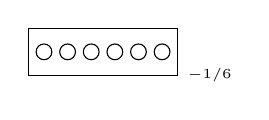
\begin{tikzpicture}
\draw (0, 0) rectangle (1.9, -0.6) node[right]{\tiny $ -1 / 6 $};
\draw (0.2, -0.3) circle (0.1);
\draw (0.5, -0.3) circle (0.1);
\draw (0.8, -0.3) circle (0.1);
\draw (1.1, -0.3) circle (0.1);
\draw (1.4, -0.3) circle (0.1);
\draw (1.7, -0.3) circle (0.1);
\end{tikzpicture}
\qquad
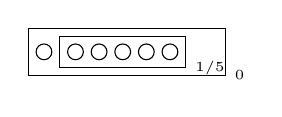
\begin{tikzpicture}
\draw (0, 0) rectangle (2.5, -0.6) node[right]{\tiny $ 0 $};
\draw (0.2, -0.3) circle (0.1);
\draw (0.4, -0.1) rectangle (2, -0.5) node[right]{\tiny $ 1 / 5 $};
\draw (0.6, -0.3) circle (0.1);
\draw (0.9, -0.3) circle (0.1);
\draw (1.2, -0.3) circle (0.1);
\draw (1.5, -0.3) circle (0.1);
\draw (1.8, -0.3) circle (0.1);
\end{tikzpicture}
\qquad
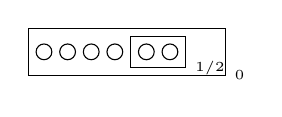
\begin{tikzpicture}
\draw (0, 0) rectangle (2.5, -0.6) node[right]{\tiny $ 0 $};
\draw (0.2, -0.3) circle (0.1);
\draw (0.5, -0.3) circle (0.1);
\draw (0.8, -0.3) circle (0.1);
\draw (1.1, -0.3) circle (0.1);
\draw (1.3, -0.1) rectangle (2, -0.5) node[right]{\tiny $ 1 / 2 $};
\draw (1.5, -0.3) circle (0.1);
\draw (1.8, -0.3) circle (0.1);
\end{tikzpicture}
$$
A simple computation shows that $ \mathfrak{f}(J_X) = (1 / t)^5 \cdot t^4 \cdot (t - 5^5 / 6^6) $.
\end{example}

\end{frame}

\begin{frame}[t]{L-functions}

Let $ k $ be finite, and let $ \rho $ be a nice \footnote{almost everywhere unramified and pure and self-dual of some integral weight} $ \ell $-adic representation of $ F $ for some fixed auxiliary prime $ \ell \ne \operatorname{char}(k) $. The \textbf{L-function} of $ \rho $ is given by
$$ L(\rho, T) := \prod_{v \in V_F} \det(1 - T \cdot \varphi_v \mid \rho^{I_v})^{-1}, $$
which is the L-function of $ J_X $ when $ \rho = \rho_{J_X} := H_{\text{\'et}}^1(\overline{X}, \mathbb{Q}_\ell) $ and $ T = q^{-s} $.

\vspace{0.5cm}

\begin{theorem}[Deligne--Grothendieck]
The numerator of the rational function $ L(\rho, T) $ is precisely $ \det(1 - T \cdot \phi_q \mid H_{\text{\'et}}^1(\overline{C}, \mathcal{F}_\rho)) $ for some constructible sheaves $ \mathcal{F}_\rho $ on $ C $, and
$$ \dim H_{\text{\'et}}^1(\overline{C}, \mathcal{F}_\rho) = \deg\mathfrak{f}(\rho) + (2g_C - 2)\dim\rho + 2\dim\rho^{\operatorname{Gal}(\overline{k}F / F)}. $$
\end{theorem}

Here, $ \mathcal{F}_\rho $ is the pushforward of a lisse sheaf on an open subset of $ C $ where $ \rho $ is unramified, and its stalk at any place $ v \in V_F $ is precisely $ \rho^{I_v} $.

\end{frame}

\begin{frame}[t]{Artin formalism}

Let $ K $ be a finite extension of $ F $. Artin's formalism gives a factorisation
$$ L(J_X / K, s) := L(\rho_{J_X / K}, q^{-s}) = \prod_{\chi \in \widehat{G}} L(\rho_{J_X} \otimes \chi, q^{-s}), $$
where $ \widehat{G} $ is the character group of the Galois closure of $ K $ over $ F $.

\vspace{0.5cm} At the level of \'etale cohomology, there are also canonical isomorphisms
$$ H_{\text{\'et}}^1(\overline{C}, \mathcal{F}_{\rho_{J_X / K}}) \cong \bigoplus_{\chi \in \widehat{G}} H_{\text{\'et}}^1(\overline{C}, \mathcal{F}_{\rho_{J_X} \otimes \chi}), $$
which respects the action of $ \phi_q $. Furthermore, if $ \widehat{G} $ can be partitioned into subsets $ o \subseteq \widehat{G} $, then there are canonical isomorphisms
$$ H_{\text{\'et}}^1(\overline{C}, \mathcal{F}_{\rho_{J_X / K}}) \cong \bigoplus_{o \subseteq \widehat{G}} H_{\text{\'et}}^1(\overline{C}, \mathcal{F}_{\rho_{J_X} \otimes (\bigoplus_{\chi \in o} \chi)}). $$

\end{frame}

\begin{frame}[t]{Geometric vanishing}

By Poincar\'e duality, the Tate twist $ H_{\text{\'et}}^1(\overline{C}, \mathcal{F}_{\rho_{J_X}(1) \otimes (\bigoplus_{\chi \in o} \chi)}) $ admits a $ \phi_q $-invariant non-degenerate symmetric bilinear pairing for any $ o \subseteq \widehat{G} $.

\vspace{0.5cm}

\begin{lemma}[Ulmer]
Let $ W_1, \dots, W_{2n} $ be finite-dimensional vector spaces with odd $ \dim W_0 $, and let $ \phi : \bigoplus_{i = 1}^{2n} W_i \to \bigoplus_{i = 1}^{2n} W_i $ be a linear map with $ \phi(W_i) = W_{i + 1} $ for all $ i \in \mathbb{Z} / 2n $, such that $ \bigoplus_{i = 1}^{2n} W_i $ admits a $ \phi_q $-invariant non-degenerate symmetric bilinear pairing that induces an isomorphism $ W_n \cong W_0^* $. Then
$$ 1 - T^{2n} \ \text{divides} \ \det(1 - T \cdot \phi \mid \textstyle\bigoplus_{i = 1}^{2n} W_i). $$
\end{lemma}

In particular, for each subset $ o \subseteq \widehat{G} $ satisfying appropriate assumptions,
$$ 1 - (qT)^{2n} \ \text{divides} \ \det(1 - T \cdot \phi_q \mid H_{\text{\'et}}^1(\overline{C}, \mathcal{F}_{\rho_{J_X} \otimes (\bigoplus_{\chi \in o} \chi)})), $$
which increments the order of vanishing of $ L(J_X / K, s) $.

\end{frame}

\begin{frame}[t]{A Frobenius action}

\begin{example}
Let $ F = \mathbb{F}_{13}(t) $, and let $ K = \mathbb{F}_{13}(\sqrt[170]{t}) $. Then $ \operatorname{Gal}(\overline{\mathbb{F}_{13}}(t) / \mathbb{F}_{13}(t)) \cong \widehat{\mathbb{Z}} $ is generated by $ \phi_{13} $, which acts naturally on $ \widehat{G} \cong \mathbb{Z} / 170 $ by
$$ \phi_{13}^i \cdot \chi := (\sigma \mapsto \chi(\phi_{13}^i(\sigma))), $$
which translates to multiplication by $ 13^{-1} \equiv -13 \mod 170 $.

\vspace{0.5cm} Let $ \widehat{G} \cong \mathbb{Z} / 170 $ be partitioned by the $ 44 $ orbits of this action given by the singletons $ \{0\} $ and $ \{85\} $, and $ \{\pm n, \pm13n\} $ for each $ n \in \mathbb{N} $.

\vspace{0.5cm} Let $ X $ be as before. If the order of $ \chi \in \widehat{G} $ is sufficiently large,
$$ \dim H_{\text{\'et}}^1(\overline{C}, \mathcal{F}_{\rho_{J_X}(1) \otimes \chi}) \equiv \deg\mathfrak{f}(\rho_{J_X}(1) \otimes \chi) \equiv \deg\mathfrak{f}(\rho_{J_X}) \mod 2, $$
which is odd. Thus the previous lemma applies, and the order of vanishing of $ L(J_X, s) $ at $ s = 1 $ is at least $ 44 - c $ for some small $ c \in \mathbb{N} $.
\end{example}

\end{frame}

\begin{frame}[t]{The Birch--Swinnerton-Dyer conjecture}

\begin{conjecture}[Birch--Swinnerton-Dyer]
The order of vanishing of $ L(J_X, s) $ at $ s = 1 $ is $ \operatorname{rk}(J_X) $, with leading term
$$ \lim_{s \to 1} \dfrac{L(J_X, s)}{(s - 1)^{\operatorname{rk}(J_X)}} = \dfrac{\operatorname{Reg}(J_X) \cdot \#\Sha(J_X) \cdot \operatorname{Tam}(J_X)}{\#\operatorname{tor}(J_X)^2}. $$
\end{conjecture}

This implicitly assumes that $ \Sha(J_X) $ is finite, which by the exact sequence
$$ 0 \to J_X(F) \otimes \mathbb{Z}_\ell \to \varprojlim_n \operatorname{Sel}_{\ell^n}(J_X) \to T_\ell\Sha(J_X) \to 0, $$
implies that the first map is an isomorphism.

\vspace{0.5cm}

\begin{theorem}[Artin--Tate, Milne, Schneider, Bauer, Kato--Trihan]
The rank conjecture is equivalent to the finiteness of $ \Sha(J_X)[\ell^\infty] $ for any prime $ \ell $, in which case the leading term conjecture also holds.
\end{theorem}

\end{frame}

\begin{frame}[t]{Invariants of surfaces}

For any nice curve $ X $ over $ F $, there is a unique irreducible proper regular relatively minimal surface $ \mathcal{X} \to C $ over $ k $, whose generic fibre is $ X $.

\vspace{0.5cm} If $ S $ is a proper regular surface over $ k $, its \textbf{Picard} and \textbf{Brauer groups} are
$$ \operatorname{Pic}(S) := H_{\text{\'et}}^1(S, \mathbb{G}_m), \qquad \operatorname{Br}(S) := H_{\text{\'et}}^2(S, \mathbb{G}_m). $$
The \textbf{N\'eron--Severi group} $ \operatorname{NS}(S) $ is the image of $ \operatorname{Pic}(S) $ in the quotient of $ \operatorname{Pic}(\overline{S}) $ by its subgroup of divisors algebraically equivalent to zero.

\vspace{0.5cm}

\begin{theorem}[Shioda--Tate]
If $ f_v $ is the number of irreducible components of the fibre $ \mathcal{X}_v $ at $ v $, then
$$ \operatorname{rk}(\operatorname{NS}(\mathcal{X})) - \operatorname{rk}(J_X) = 2 + \sum_v (f_v - 1). $$
\end{theorem}

\vspace{-0.5cm}

\begin{theorem}[Grothendieck]
There is a canonical isomorphism $ \operatorname{Br}(\mathcal{X}) \xrightarrow{\sim} \Sha(J_X) $.
\end{theorem}

\end{frame}

\begin{frame}[t]{The Tate conjecture}

Analogously to $ J_X $, there is an exact sequence
$$ 0 \to \operatorname{NS}(\mathcal{X}) \otimes \mathbb{Z}_\ell \xrightarrow{c_\ell} \varprojlim_n H_{\text{\'et}}^2(\overline{\mathcal{X}}, \mu_{\ell^n})^{G_k} \to T_\ell\operatorname{Br}(\mathcal{X}) \to 0, $$
so the finiteness of $ \Sha(J_X)[\ell^\infty] $ reduces to $ c_\ell $ being an isomorphism.

\vspace{0.5cm}

\begin{conjecture}[Tate]
The cycle class map $ c_\ell $ is an isomorphism for any prime $ \ell $. Equivalently,
$$ \operatorname{rk}(\operatorname{NS}(\mathcal{X})) = -\operatorname{ord}_{s = 1} \zeta(\mathcal{X}, s). $$
\end{conjecture}

In particular, this is independent of $ \ell $. It turns out that
$$ -\operatorname{ord}_{s = 1} \zeta(\mathcal{X}, s) - \operatorname{ord}_{s = 1} L(J_X, s) = 2 + \sum_v (f_v - 1), $$
so the rank conjecture is equivalent to the Tate conjecture.

\end{frame}

\begin{frame}[t]{A Delsarte surface}

Tate's conjecture is known to hold for rational surfaces, abelian surfaces, elliptic K3 surfaces, and surfaces dominated by a product of nice curves.

\begin{example}
Let $ X $ be as before. It defines a \emph{Delsarte} surface $ \mathcal{X} \subseteq \mathbb{P}_{[z : t : x : y]}^3 $ given by
$$ z^4y^2 - x^6 - zx^5 - z^5t = 0, $$
which is dominated by the \emph{Fermat} surface $ S \subseteq \mathbb{P}_{[y_0 : y_1 : y_2 : y_3]}^3 $ given by
$$ y_0^2 + y_1^2 + y_2^2 + y_3^2 = 0, $$
by the rational map $ S \to \mathcal{X} $ given by
$$ [y_0 : y_1 : y_2 : y_3] \mapsto \left[\dfrac{y_2^{12}}{y_1^{10}} : y_3^2 : \dfrac{y_2^{10}}{y_1^8} : \dfrac{5y_0y_2^6}{y_1^5}\right]. $$
In particular, the Tate conjecture holds for $ \mathcal{X} $. Thus the rank conjecture, and hence the full Birch--Swinnerton-Dyer conjecture, holds for $ J_X $.
\end{example}

\end{frame}

\end{document}